\documentclass[aspectratio=169,11pt]{beamer}

\setbeamertemplate{navigation symbols}{}
\setbeamertemplate{blocks}[rounded][shadow=false]
\setbeamertemplate{itemize item}{\color{accentB}$\blacktriangleright$}
\setbeamertemplate{itemize subitem}{\color{accentC}$\bullet$}

\usepackage[utf8]{inputenc}
\usepackage[T1]{fontenc}
\usepackage{booktabs}
\usepackage{tikz}
\usepackage{graphicx}
\usepackage{array}
\usepackage{tabularx}
\usetikzlibrary{positioning, arrows.meta, shapes.geometric, calc, shadows}

% ── Palette ───────────────────────────────────────────────────────────────────
\definecolor{bgSoft}{HTML}{FAFBFC}
\definecolor{ink}{HTML}{121212}
\definecolor{accentA}{HTML}{0B6E4F}
\definecolor{accentB}{HTML}{D9480F}
\definecolor{accentC}{HTML}{0059B3}
\definecolor{muted}{HTML}{5B5B5B}
\definecolor{cardBg}{HTML}{FFFFFF}
\definecolor{lineSoft}{HTML}{DEE2E6}
\definecolor{critRed}{HTML}{C53030}
\definecolor{modOrange}{HTML}{C05621}
\definecolor{routGreen}{HTML}{276749}

\setbeamercolor{background canvas}{bg=bgSoft}
\setbeamercolor{normal text}{fg=ink,bg=bgSoft}
\setbeamercolor{title}{fg=ink}
\setbeamercolor{frametitle}{fg=ink,bg=bgSoft}
\setbeamercolor{item}{fg=accentB}
\setbeamercolor{block title}{fg=white,bg=accentC}
\setbeamercolor{block body}{fg=ink,bg=cardBg}
\setbeamercolor{section in toc}{fg=ink}
\setbeamercolor{subsection in toc}{fg=muted}

\setbeamerfont{title}{series=\bfseries,size=\Huge}
\setbeamerfont{frametitle}{series=\bfseries,size=\large}
\setbeamerfont{block title}{series=\bfseries,size=\small}

% ── Frame title with rule ─────────────────────────────────────────────────────
\makeatletter
\setbeamertemplate{frametitle}{%
  \vspace{0.25em}
  \begin{beamercolorbox}[wd=\paperwidth,leftskip=0.8em,rightskip=0.8em]{frametitle}
    {\usebeamerfont{frametitle}\insertframetitle}
    \ifx\insertframesubtitle\@empty\else
      \par\vspace{0.1em}{\small\color{muted}\insertframesubtitle}
    \fi
  \end{beamercolorbox}
  \vspace{-0.4em}
  \begin{tikzpicture}
    \draw[line width=0.6pt, color=lineSoft] (0,0) -- (\paperwidth,0);
  \end{tikzpicture}
}
\makeatother

% ── Footline ─────────────────────────────────────────────────────────────────
\setbeamerfont{footline}{size=\scriptsize}
\setbeamertemplate{footline}{%
  \leavevmode
  \hbox{%
    \begin{beamercolorbox}[wd=.75\paperwidth,ht=2.5ex,dp=1ex,leftskip=1em]{author in head/foot}%
      \color{muted}PneumoScan \textbullet{} Anis Aissani \textbullet{} L3 Informatique, Univ. Rouen Normandie
    \end{beamercolorbox}%
    \begin{beamercolorbox}[wd=.25\paperwidth,ht=2.5ex,dp=1ex,rightskip=1em plus1fil]{date in head/foot}%
      \color{muted}\hfill\insertframenumber\,/\,\inserttotalframenumber
    \end{beamercolorbox}%
  }%
  
\begin{tikzpicture}[remember picture,overlay]
    \fill[accentA] (0,0) rectangle (\paperwidth,0.05);
  \end{tikzpicture}
}

% ── Custom commands ───────────────────────────────────────────────────────────
\newcommand{\badge}[3]{%
  \tikz[baseline=(t.base)]\node[fill=#1!15,draw=#1!40,rounded corners=2pt,
    inner sep=2pt,font=\scriptsize\bfseries,text=#1](t){#3};}
\newcommand{\CRIT}{\badge{critRed}{critRed}{CRITICAL}}
\newcommand{\MOD}{\badge{modOrange}{modOrange}{MODERATE}}
\newcommand{\ROUT}{\badge{routGreen}{routGreen}{ROUTINE}}

\title[PneumoScan]{%
  \vspace{0.3em}%
  PneumoScan\\[0.2em]
  \large Aide au triage automatise des radiographies thoraciques%
}
\author{Anis Aissani}
\institute{Universite de Rouen Normandie --- L3 Informatique}
\date{2025 -- 2026}

% =============================================================================
\begin{document}
% =============================================================================

% ── Title slide ───────────────────────────────────────────────────────────────
\begin{frame}[plain]
\begin{tikzpicture}[remember picture,overlay]
  % Background accents
  \fill[accentC!8]  (current page.north west)
    rectangle ([xshift=7cm,yshift=-3cm]current page.north west);
  \fill[accentB!12] ([xshift=-4.5cm,yshift=2.2cm]current page.south east)
    rectangle (current page.south east);
  % Green bar
  \fill[accentA]    (current page.south west)
    rectangle ([xshift=\paperwidth,yshift=0.22cm]current page.south west);
  % Top accent line
  \draw[line width=2.5pt, accentA]
    ([xshift=1cm,yshift=-1.1cm]current page.north west)
    -- ([xshift=8cm,yshift=-1.1cm]current page.north west);
\end{tikzpicture}
\titlepage
\vspace{-0.5em}
\begin{center}
  \small\color{muted}
  Encadrant : Prof.\ C.\ Petitjean \quad\textbullet\quad
  Binome : Mohammed Elakef Zenagui
\end{center}
\end{frame}

% ── Plan ──────────────────────────────────────────────────────────────────────
\begin{frame}{Plan}
\tableofcontents
\end{frame}

% =============================================================================
\section{Contexte et problematique}
% =============================================================================

\begin{frame}{Contexte}
\begin{columns}[T,onlytextwidth]
\column{0.55\textwidth}
\begin{itemize}
  \item La pneumonie cause \textbf{2,5 millions de deces} par an dans le monde.
  \item Diagnostic repose sur la lecture de radiographies thoraciques.
  \item Files d'attente traitees en FIFO : un cas grave peut attendre trop longtemps.
\end{itemize}
\vspace{0.8em}
\begin{block}{Objectif}
Developper un outil de triage automatise qui classe chaque radiographie
en priorite clinique, tout en garantissant la tracabilite et la securite des acces.
\end{block}

\column{0.42\textwidth}
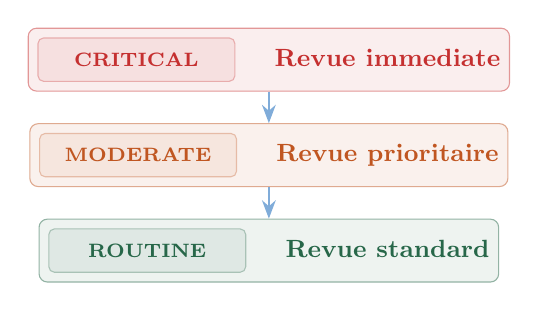
\begin{tikzpicture}[every node/.style={font=\small}, node distance=0.4cm]
  \node[draw=critRed!50, fill=critRed!8, rounded corners=3pt,
        minimum width=2.5cm, minimum height=0.55cm, text=critRed,
        font=\small\bfseries] (c) {\CRIT{} \quad Revue immediate};
  \node[draw=modOrange!50, fill=modOrange!8, rounded corners=3pt,
        minimum width=2.5cm, minimum height=0.55cm, text=modOrange,
        font=\small\bfseries, below=of c] (m) {\MOD{} \quad Revue prioritaire};
  \node[draw=routGreen!50, fill=routGreen!8, rounded corners=3pt,
        minimum width=2.5cm, minimum height=0.55cm, text=routGreen,
        font=\small\bfseries, below=of m] (r) {\ROUT{} \quad Revue standard};
  \draw[-{Stealth},thick,accentC!50] (c) -- (m);
  \draw[-{Stealth},thick,accentC!50] (m) -- (r);
\end{tikzpicture}
\end{columns}
\end{frame}

\begin{frame}{Problematique et organisation du projet}
\begin{columns}[T,onlytextwidth]
\column{0.50\textwidth}
\textbf{Problematique}\\[4pt]
Comment integrer un modele ML pre-entraine dans une architecture web
securisee garantissant tracabilite et rejet des entrees hors-distribution ?

\vspace{0.8em}
\textbf{Repartition du travail}
\begin{itemize}
  \item \textcolor{accentA}{\textbf{Binome}} : entrainement et validation des modeles
        (HOG, LBP, Haralick, ResNet, EfficientNet)
  \item \textcolor{accentC}{\textbf{Mon apport}} : architecture logicielle complete ---
        API, interface, securite, deploiement
\end{itemize}

\column{0.47\textwidth}
\begin{block}{Methodologie : UP adapte}
\begin{tabular}{@{}l l@{}}
\textbf{Inception}    & 2 sem. \\
\textbf{Elaboration}  & 4 sem. \\
\textbf{Construction} & 8 sem. \\
\textbf{Transition}   & 2 sem. \\
\end{tabular}
\end{block}
\vspace{0.5em}
\textcolor{muted}{\small Prototype academique, non certifie dispositif medical}
\end{columns}
\end{frame}

% =============================================================================
\section{Architecture technique}
% =============================================================================

\begin{frame}{Vue d'ensemble}
\centering
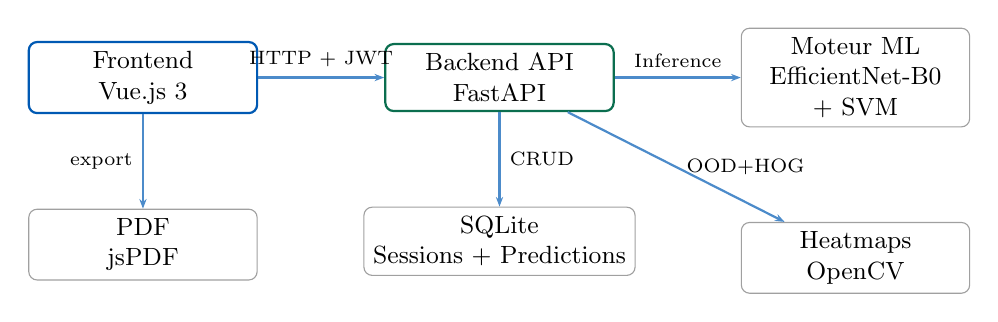
\begin{tikzpicture}[
  node distance=1.6cm,
  box/.style={rectangle, draw=ink!40, rounded corners=3pt,
              minimum width=2.9cm, minimum height=0.85cm,
              align=center, fill=white, font=\small},
  arr/.style={-{Stealth[length=3.5pt]}, thick, draw=accentC!70}
]
\node[box, draw=accentC, thick] (fe) {Frontend\\Vue.js 3};
\node[box, right=of fe, draw=accentA, thick] (api) {Backend API\\FastAPI};
\node[box, right=of api] (ml) {Moteur ML\\EfficientNet-B0\\+ SVM};
\node[box, below=1.2cm of api] (db) {SQLite\\Sessions + Predictions};
\node[box, below=1.2cm of fe] (pdf) {PDF\\jsPDF};
\node[box, below=1.2cm of ml] (heat) {Heatmaps\\OpenCV};

\draw[arr] (fe)  -- node[above,font=\scriptsize]{HTTP + JWT} (api);
\draw[arr] (api) -- node[above,font=\scriptsize]{Inference} (ml);
\draw[arr] (api) -- node[right,font=\scriptsize]{CRUD} (db);
\draw[arr] (api) -- node[right,font=\scriptsize]{OOD+HOG} (heat);
\draw[arr] (fe)  -- node[left,font=\scriptsize]{export} (pdf);
\end{tikzpicture}
\end{frame}

\begin{frame}{Pipeline d'analyse et architecture modulaire}
\begin{columns}[T,onlytextwidth]
\column{0.50\textwidth}
\textbf{Pipeline image}\\[4pt]
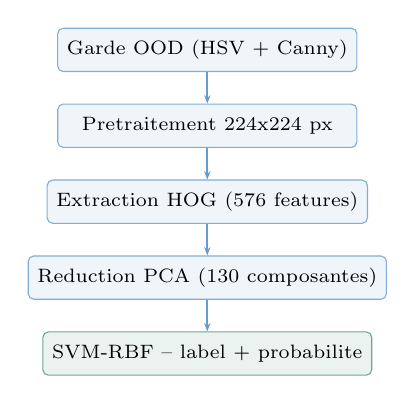
\begin{tikzpicture}[
  pstep/.style={rectangle, rounded corners=2pt, draw=accentC!50,
                fill=accentC!6, minimum width=3.8cm,
                minimum height=0.55cm, font=\scriptsize, align=center},
  arr/.style={-{Stealth[length=3pt]}, thick, accentC!60},
  node distance=0.4cm
]
\node[pstep] (ood)  {Garde OOD (HSV + Canny)};
\node[pstep, below=of ood]  (pre)  {Pretraitement 224x224 px};
\node[pstep, below=of pre]  (feat) {Extraction HOG (576 features)};
\node[pstep, below=of feat] (pca)  {Reduction PCA (130 composantes)};
\node[pstep, below=of pca, draw=accentA!60, fill=accentA!8]
     (svm) {SVM-RBF -- label + probabilite};
\draw[arr] (ood) -- (pre);
\draw[arr] (pre) -- (feat);
\draw[arr] (feat) -- (pca);
\draw[arr] (pca) -- (svm);
\end{tikzpicture}

\column{0.47\textwidth}
\textbf{Modules backend}\\[4pt]
\begin{tabular}{@{}l l@{}}
\texttt{main.py}      & Routes FastAPI \\
\texttt{services.py}  & Logique metier \\
\texttt{predictor.py} & Pipeline ML \\
\texttt{database.py}  & SQLite + triage \\
\texttt{auth.py}      & JWT / RBAC \\
\texttt{utils.py}     & Validation \\
\end{tabular}

\vspace{0.8em}
\textbf{Modele retenu}\\
EfficientNet-B0 + SVM\\
\textcolor{accentA}{\textbf{Accuracy 86.2\% \quad F1 88.4\%}}\\[4pt]
\textcolor{muted}{\scriptsize Fallback deploye : HOG + PCA + SVM (F1 81.4\%)}
\end{columns}
\end{frame}

\begin{frame}{Securite et tracabilite}
\begin{columns}[T,onlytextwidth]
\column{0.50\textwidth}
\textbf{Authentification JWT / RBAC}
\begin{itemize}
  \item 2 roles : \texttt{radiologist} et \texttt{admin}
  \item Token HS256, TTL 8h (1 shift hospitalier)
  \item Mots de passe haches bcrypt
  \item Stockage dans \texttt{sessionStorage} uniquement
\end{itemize}
\vspace{0.5em}
\textbf{Sessions anti-zombie}
\begin{itemize}
  \item A chaque reconnexion, les sessions ouvertes precedentes sont
        automatiquement cloturees
  \item Chaque prediction est tracee : operateur, horodatage, session
\end{itemize}

\column{0.47\textwidth}
\textbf{Regle de triage}
\[
\text{\CRIT} \; = \hat{y}=P \;\land\; p > 0.85
\]
\[
\text{\MOD} \; = \hat{y}=P \;\land\; 0.15 \!\le\! p \!\le\! 0.85
\]
\[
\text{\ROUT} \; = \hat{y}=N \;\lor\; p < 0.15
\]
\vspace{0.3em}
\textbf{Anonymisation RGPD}\\
Masquage noir irréversible des coins\\
(zones PACS contenant les donnees patient)
\end{columns}
\end{frame}

% =============================================================================
\section{Demonstration de l'application}
% =============================================================================

\begin{frame}{Connexion et ouverture de session}
\begin{columns}[T,onlytextwidth]
\column{0.52\textwidth}
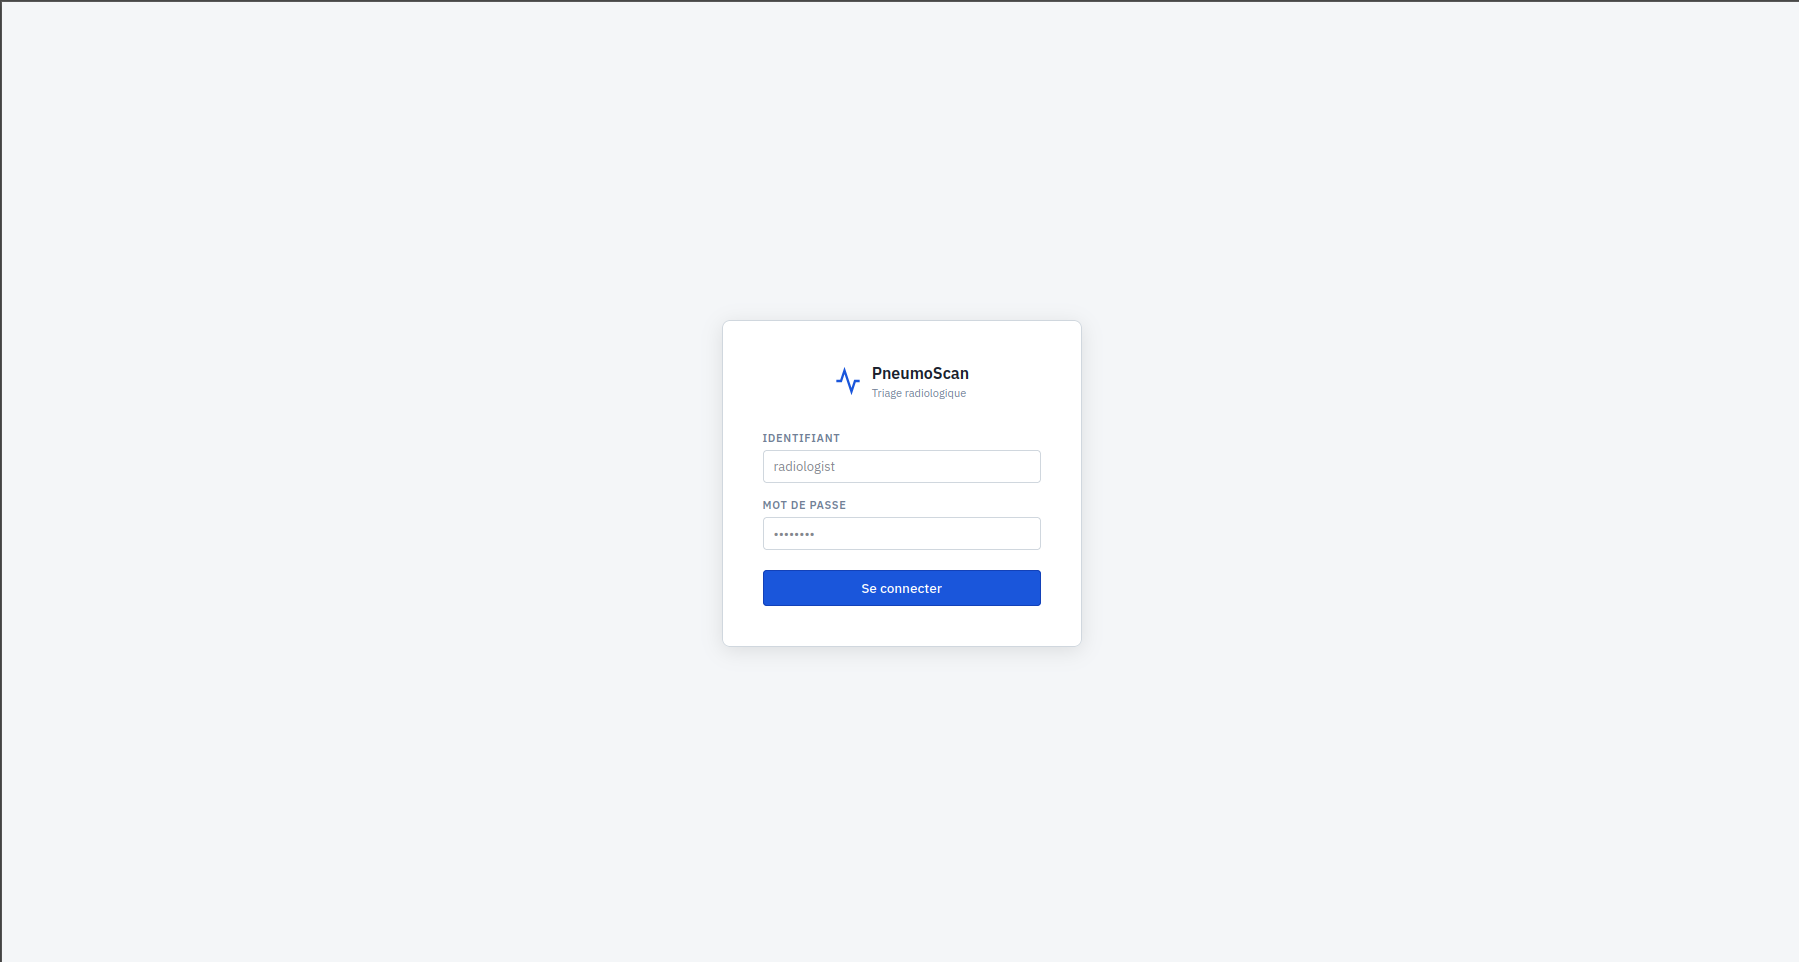
\includegraphics[width=\linewidth]{assets/ui_login.png}

\column{0.45\textwidth}
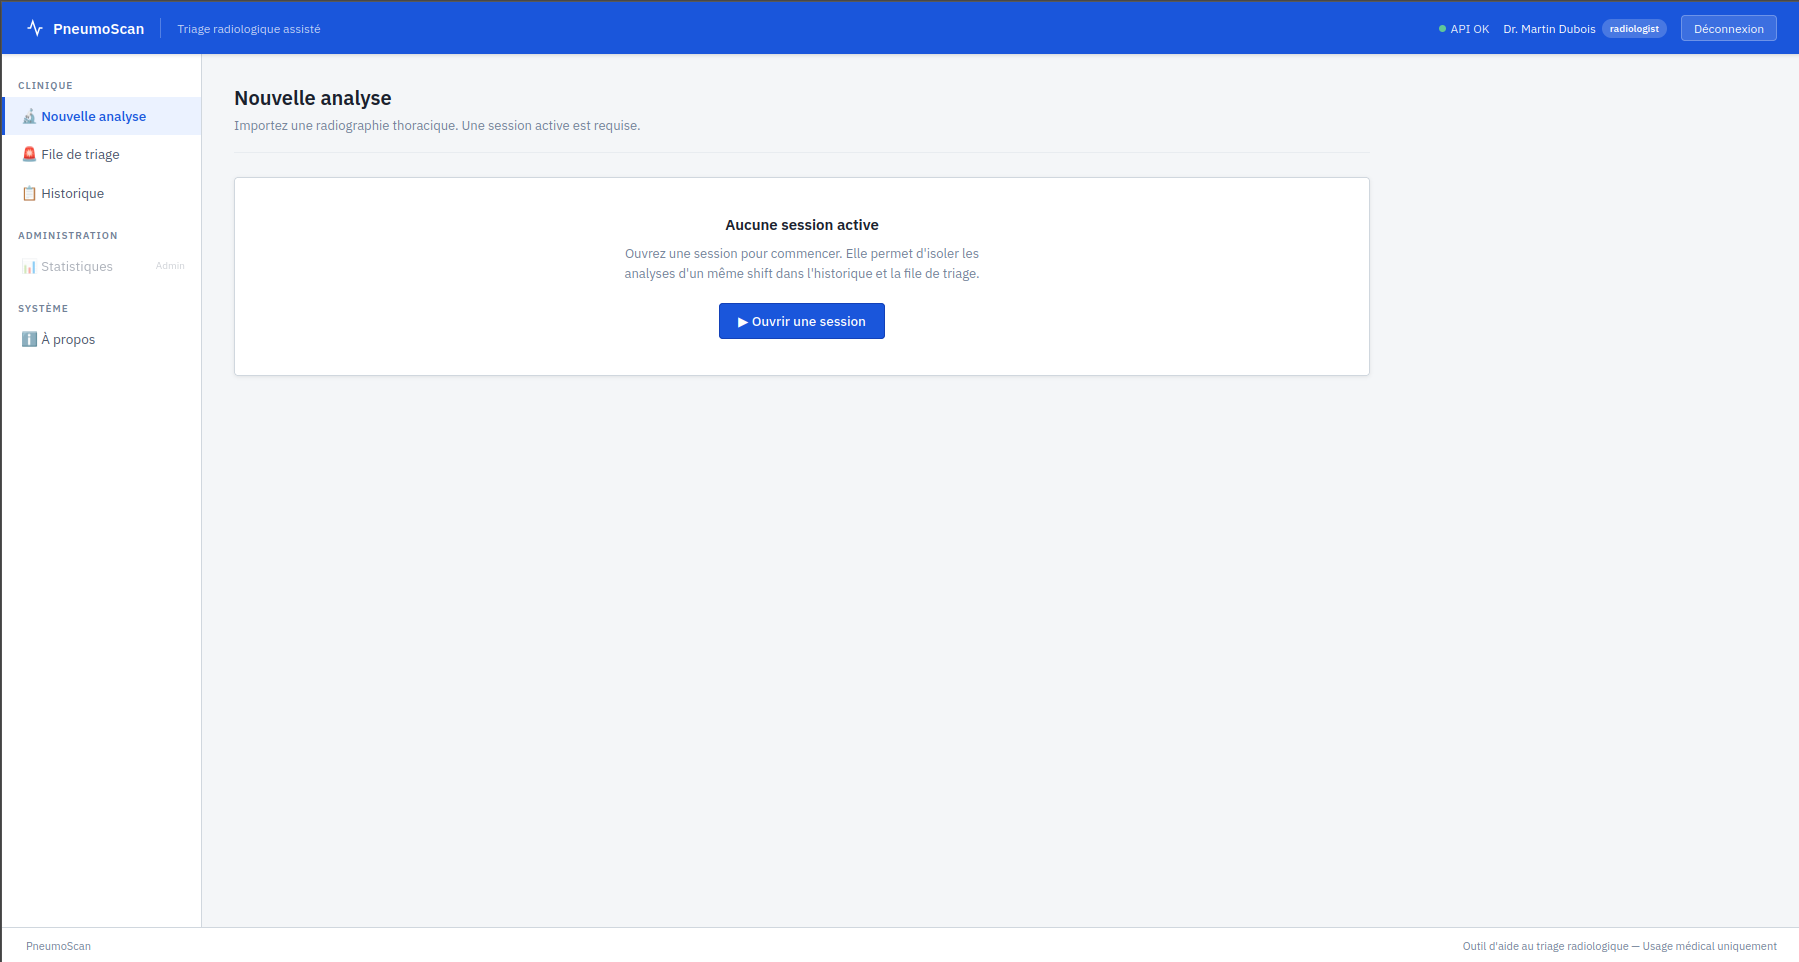
\includegraphics[width=\linewidth]{assets/ui_new_analysis_no_session.png}
\vspace{0.5em}
\begin{itemize}
  \item Connexion securisee par JWT
  \item Sans session active, l'analyse est bloquee
  \item Chaque session rattache les analyses a un shift et un operateur
\end{itemize}
\end{columns}
\end{frame}

\begin{frame}{Analyse radiographique}
\centering
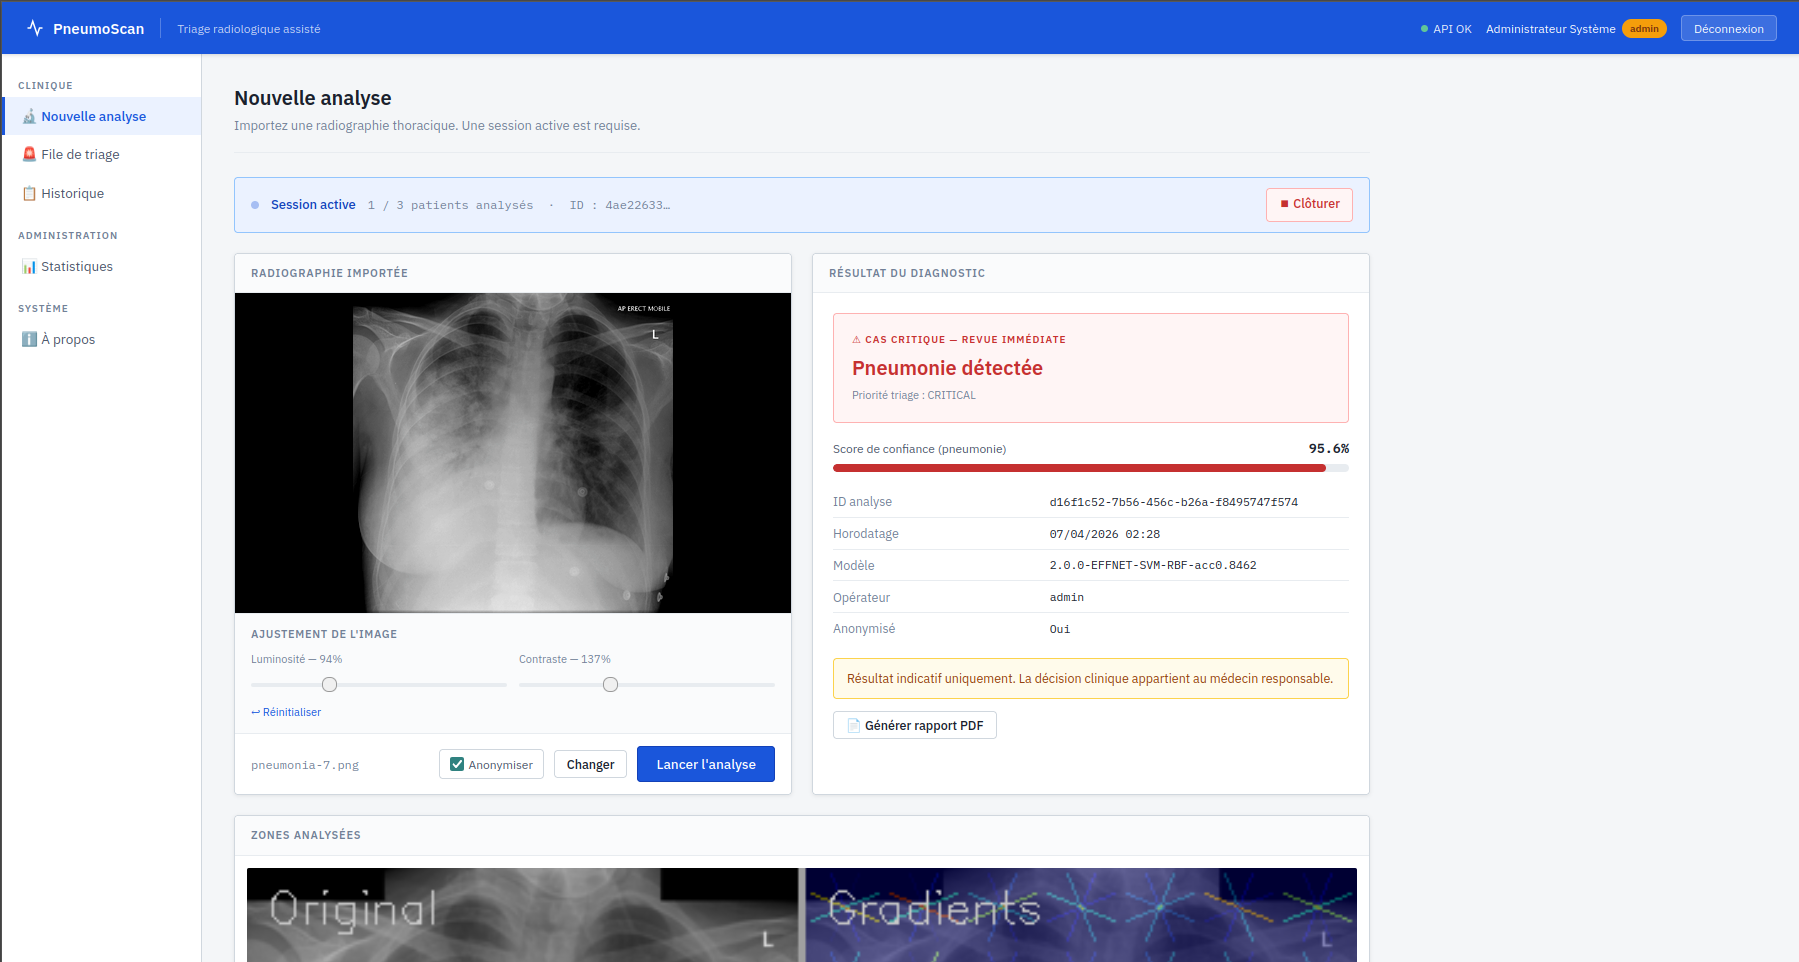
\includegraphics[width=0.88\linewidth,height=0.75\textheight,keepaspectratio]{assets/ui_analysis_result.png}
\end{frame}

\begin{frame}{Explicabilite visuelle : zones analysees}
\centering
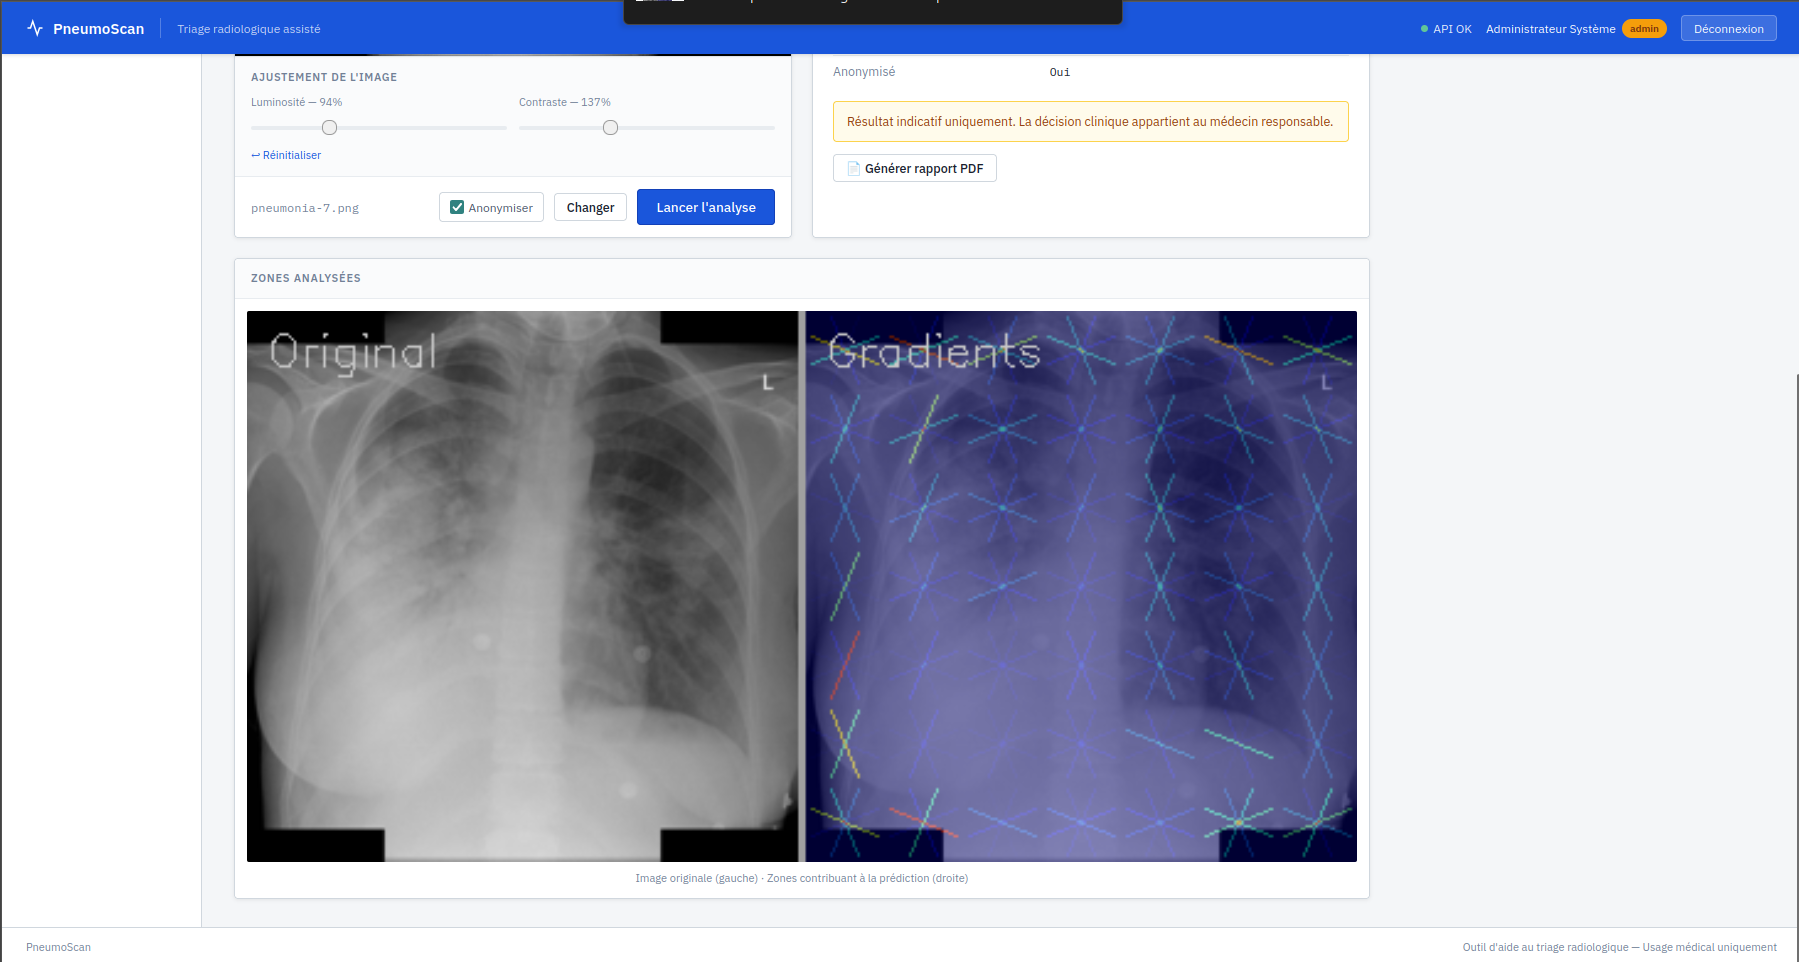
\includegraphics[width=0.90\linewidth,height=0.78\textheight,keepaspectratio]{assets/ui_analyzed_zones.png}
\end{frame}

\begin{frame}{Rapport PDF genere automatiquement}
\centering
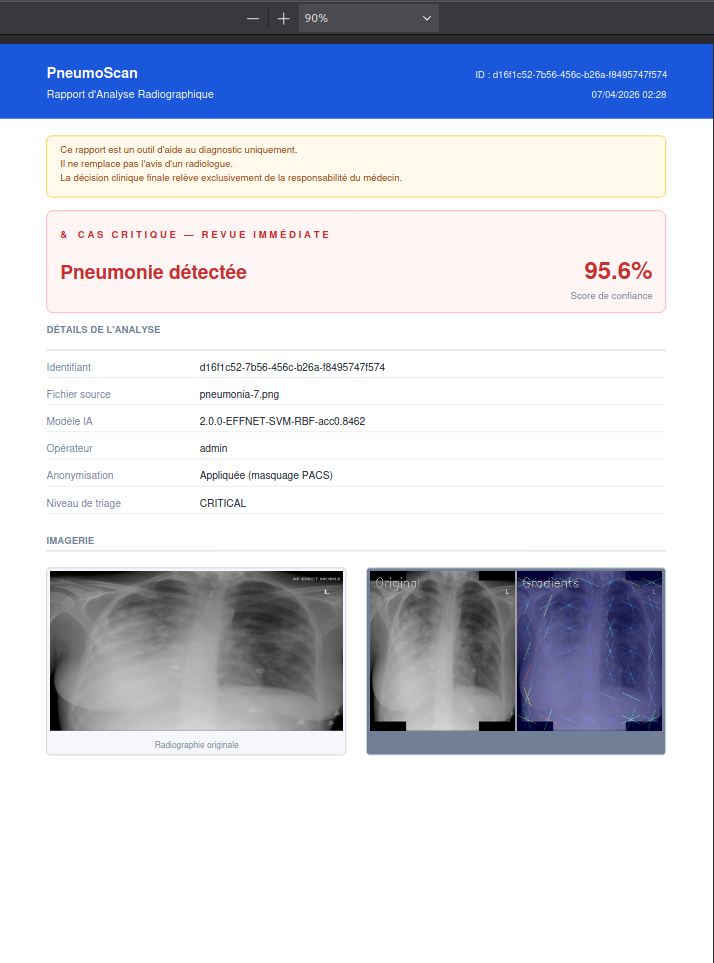
\includegraphics[width=0.72\linewidth,height=0.80\textheight,keepaspectratio]{assets/ui_pdf_report.png}
\end{frame}

\begin{frame}{File de triage et historique}
\begin{columns}[T,onlytextwidth]
\column{0.55\textwidth}
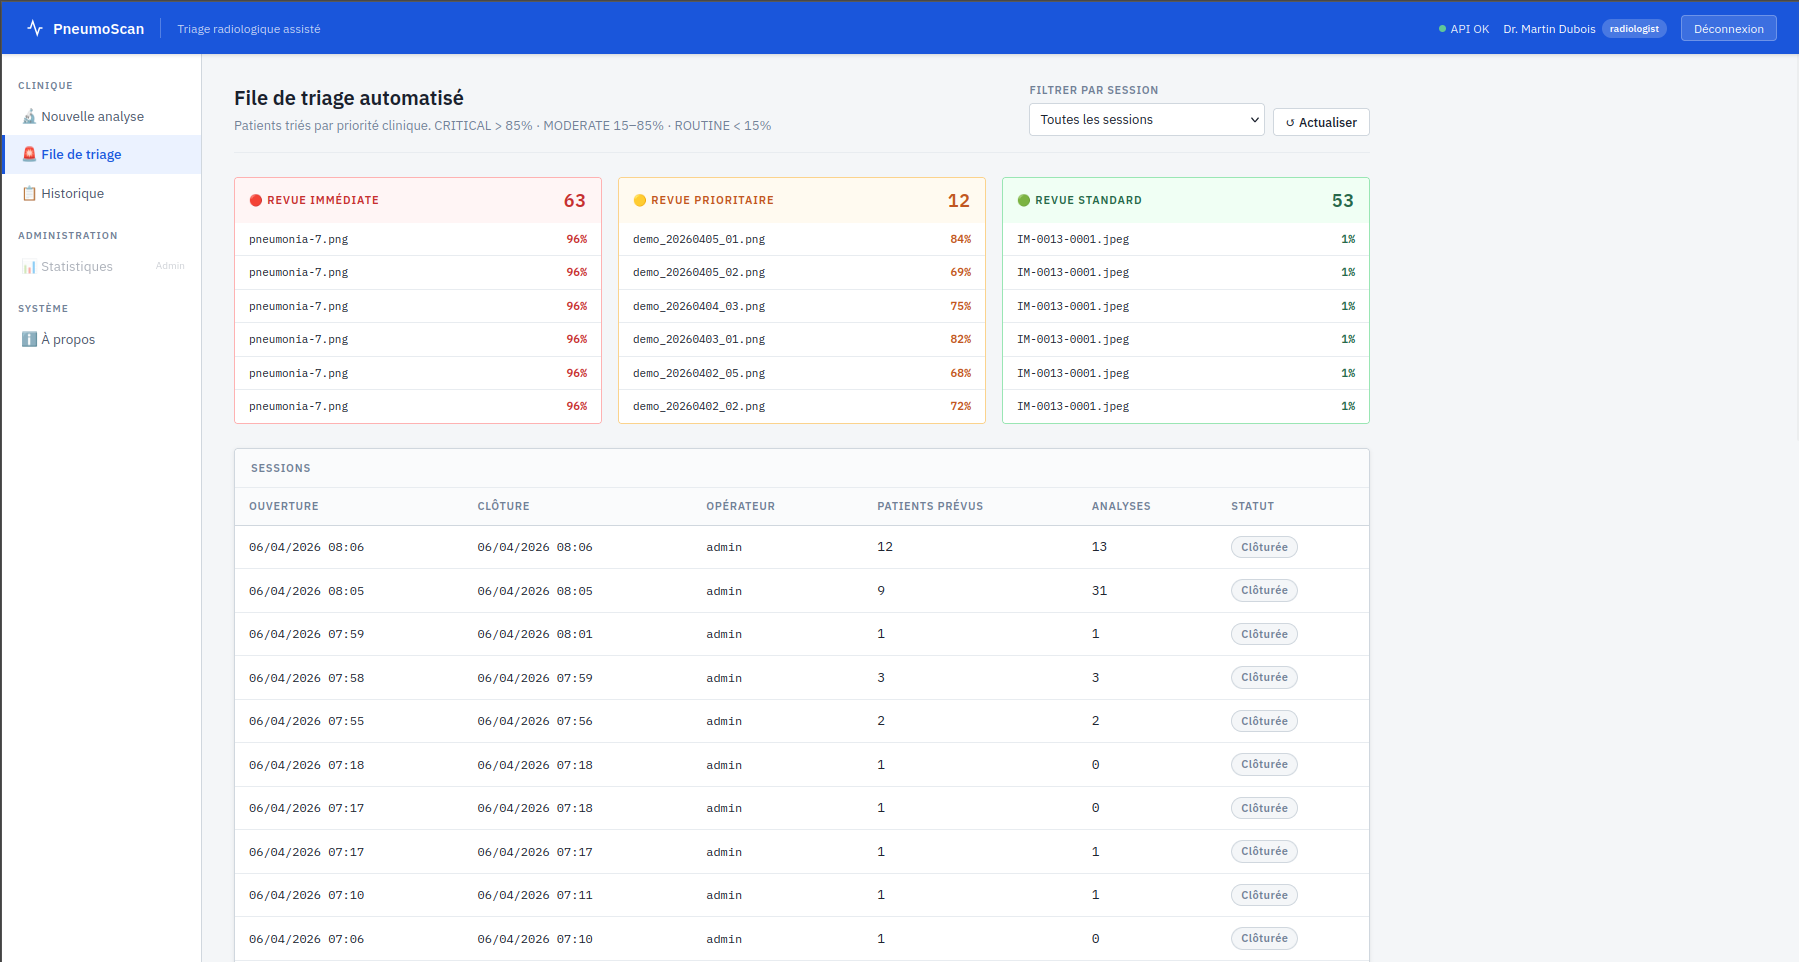
\includegraphics[width=\linewidth,height=0.72\textheight,keepaspectratio]{assets/ui_triage_queue.png}

\column{0.42\textwidth}
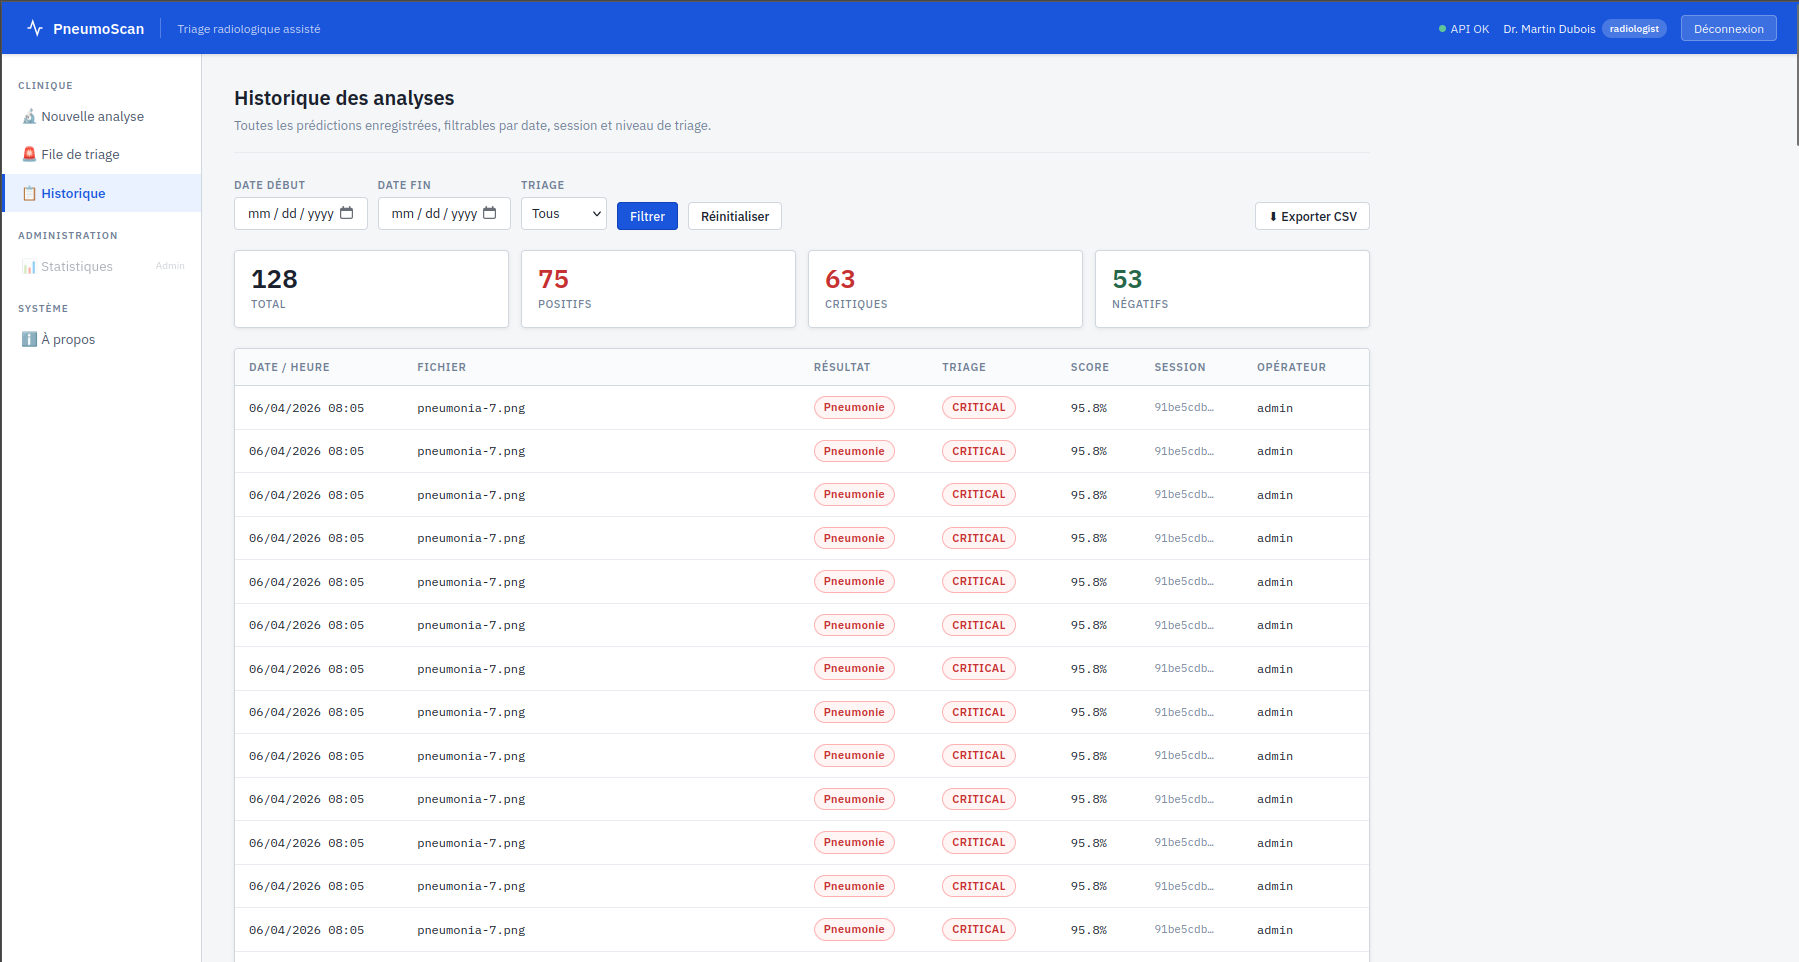
\includegraphics[width=\linewidth]{assets/ui_history.png}
\vspace{0.5em}
\begin{itemize}
  \item 3 colonnes : \CRIT{} / \MOD{} / \ROUT{}
  \item Historique filtrable + export CSV
\end{itemize}
\end{columns}
\end{frame}

\begin{frame}{Tableau de bord et page a propos}
\begin{columns}[T,onlytextwidth]
\column{0.55\textwidth}
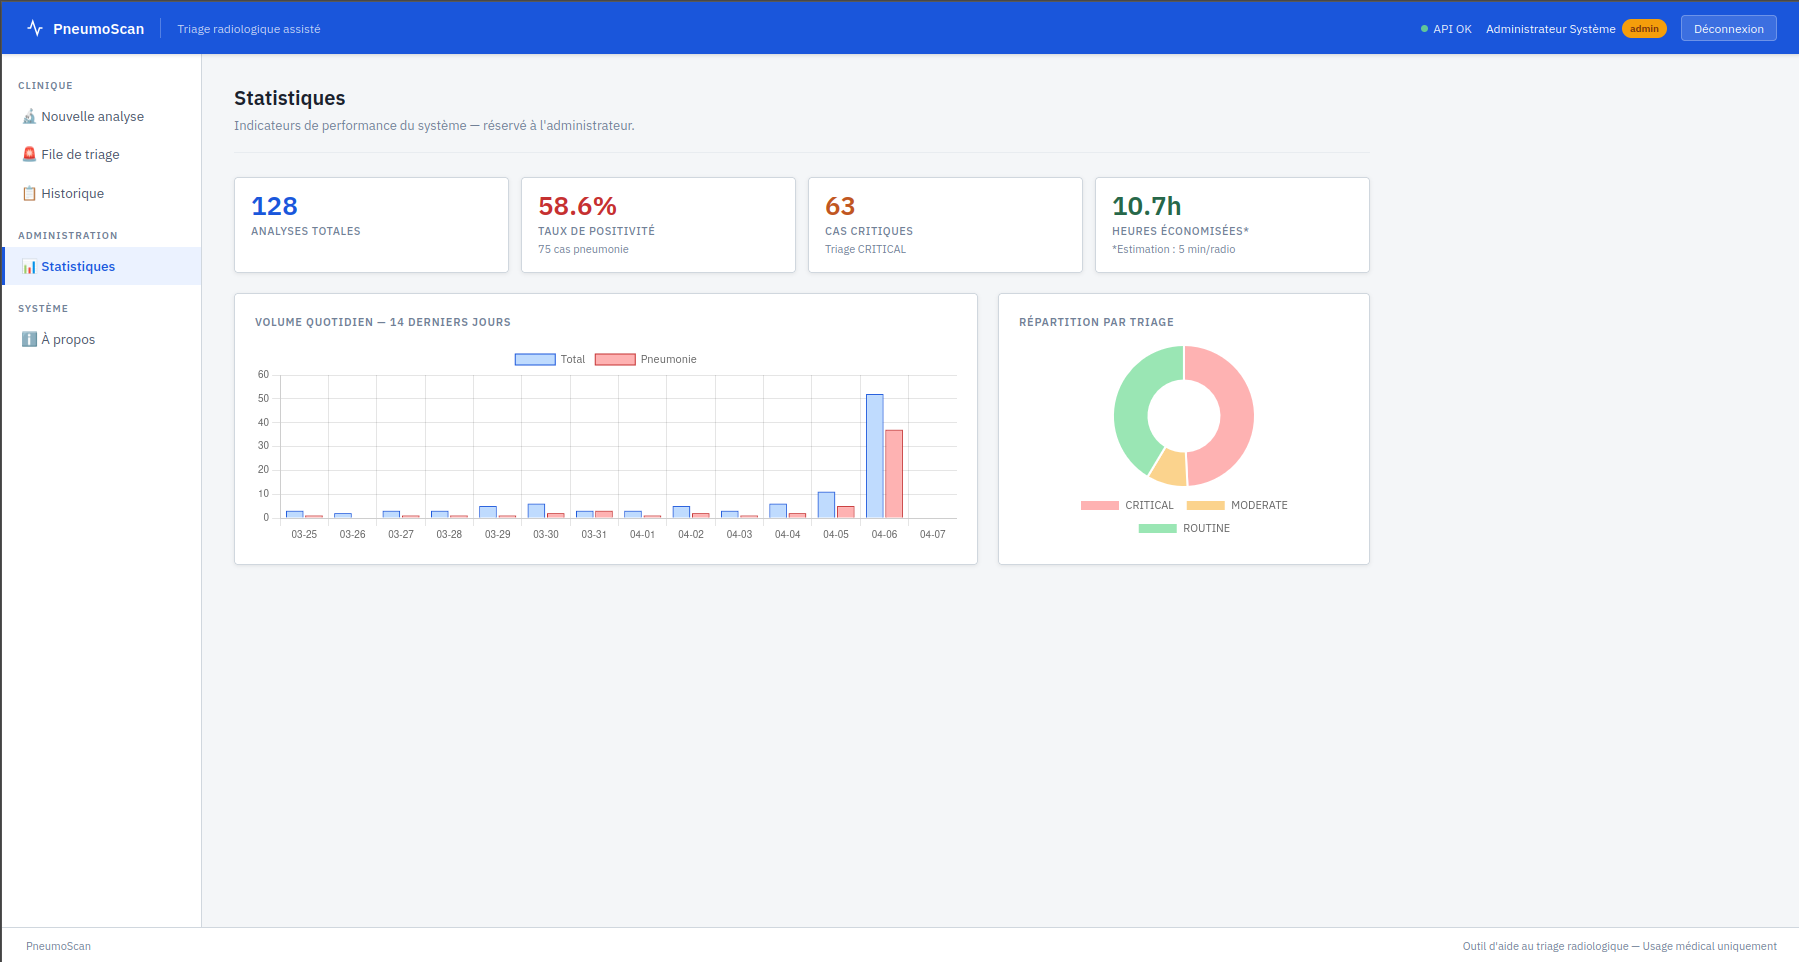
\includegraphics[width=\linewidth,height=0.40\textheight,keepaspectratio]{assets/ui_admin_stats.png}
\vspace{0.3em}
\begin{itemize}
  \item Reserve au role \texttt{admin}
  \item Volume, positivite, repartition triage
  \item Estimation heures economisees
\end{itemize}

\column{0.42\textwidth}
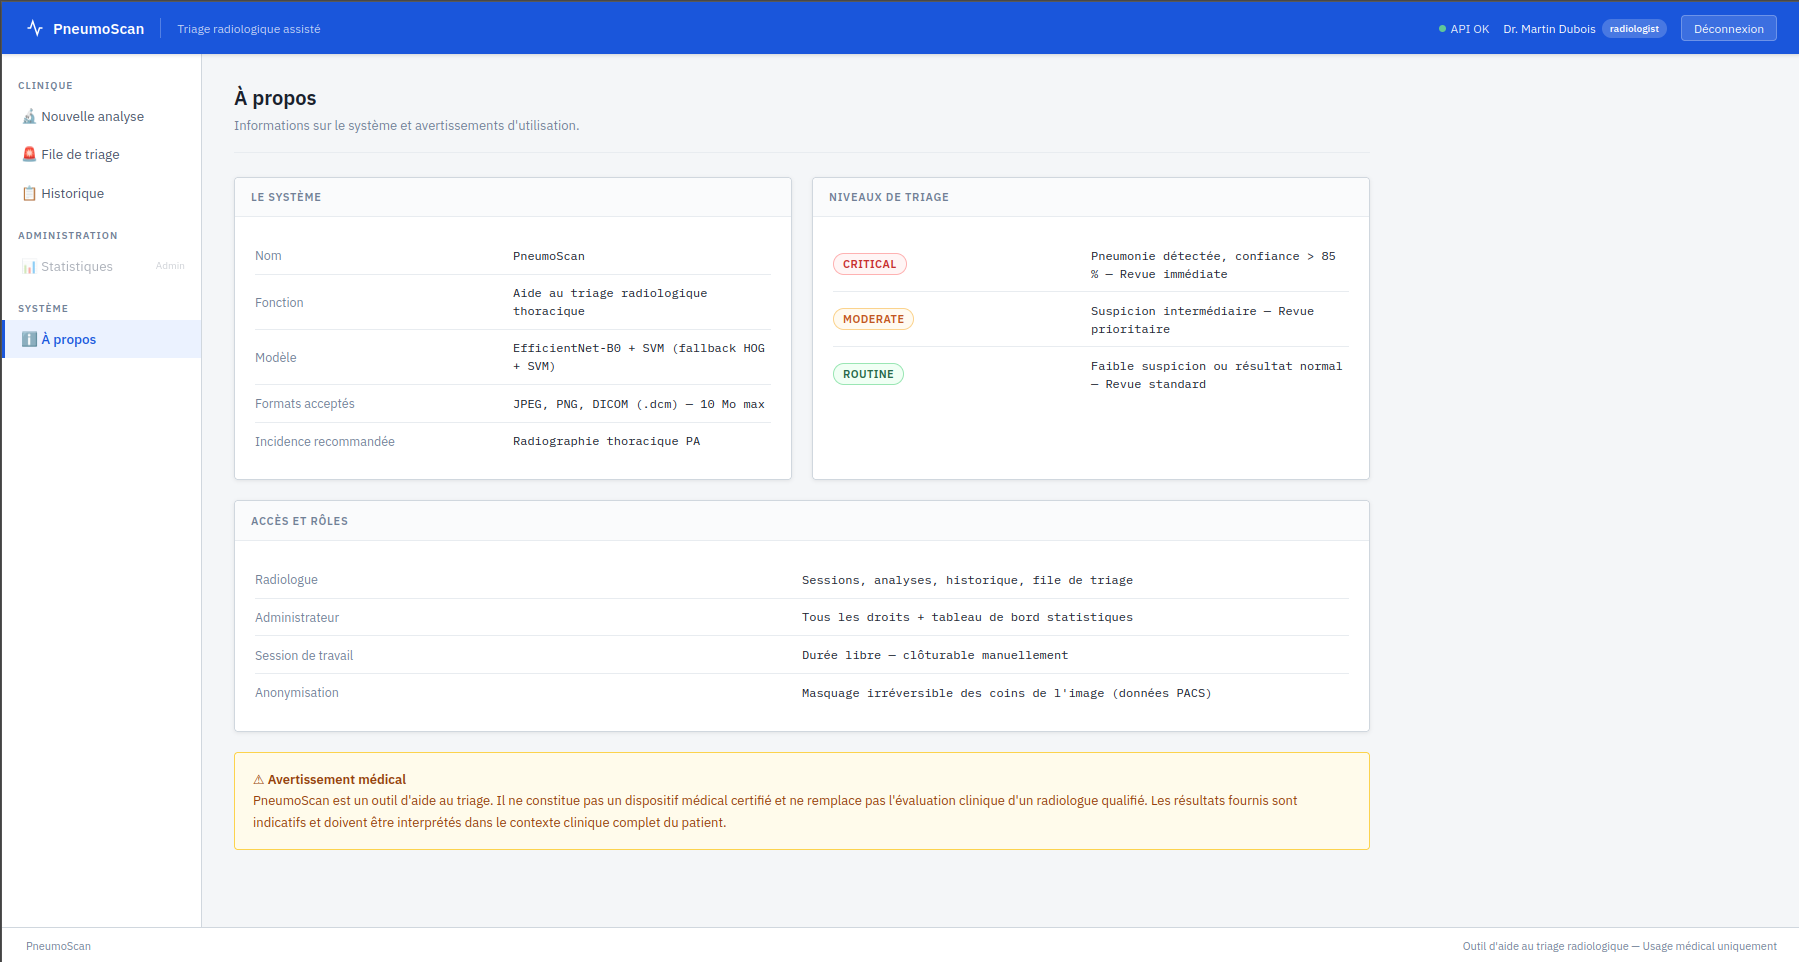
\includegraphics[width=\linewidth,height=0.40\textheight,keepaspectratio]{assets/ui_about.png}
\vspace{0.3em}
\begin{itemize}
  \item Perimetre d'usage clairement affiche
  \item Avertissement medical integre
\end{itemize}
\end{columns}
\end{frame}

% =============================================================================
\section{Demonstration en direct}
% =============================================================================

\begin{frame}[c]{}
\centering
\begin{tikzpicture}[remember picture, overlay]
  \fill[accentC!8] (current page.north west) rectangle (current page.south east);
\end{tikzpicture}
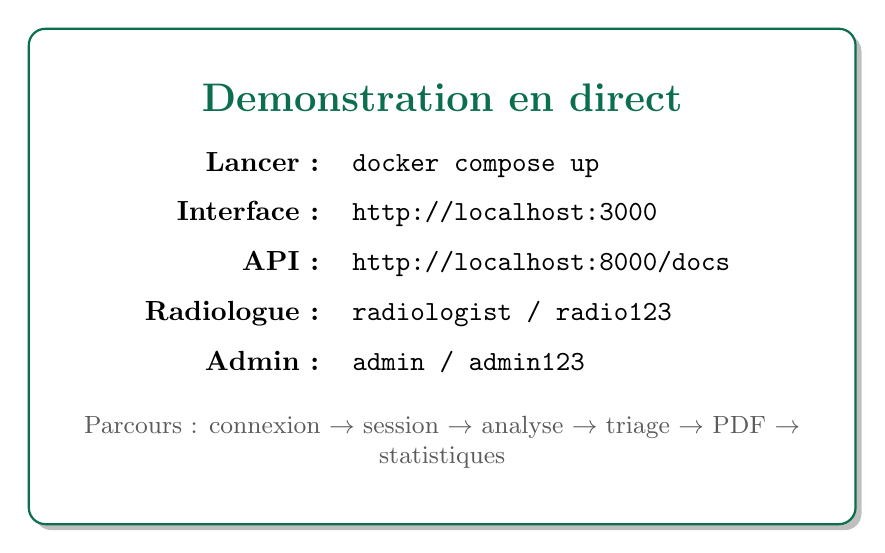
\begin{tikzpicture}
  \node[draw=accentA, thick, rounded corners=6pt,
        fill=white, inner sep=20pt, drop shadow] {
    \begin{minipage}{0.75\textwidth}
      \centering
      {\Large\bfseries\color{accentA} Demonstration en direct}\\[12pt]
      \begin{tabular}{r l}
        \textbf{Lancer :} & \texttt{docker compose up} \\[6pt]
        \textbf{Interface :} & \texttt{http://localhost:3000} \\[6pt]
        \textbf{API :}       & \texttt{http://localhost:8000/docs} \\[6pt]
        \textbf{Radiologue :} & \texttt{radiologist / radio123} \\[6pt]
        \textbf{Admin :}      & \texttt{admin / admin123} \\
      \end{tabular}
      \vspace{12pt}\\
      \color{muted}\small
      Parcours : connexion $\rightarrow$ session $\rightarrow$ analyse $\rightarrow$
      triage $\rightarrow$ PDF $\rightarrow$ statistiques
    \end{minipage}
  };
\end{tikzpicture}
\end{frame}

% =============================================================================
\section{Qualite et bilan}
% =============================================================================

\begin{frame}{Tests et qualite logicielle}
\begin{columns}[T,onlytextwidth]
\column{0.50\textwidth}
\textbf{Suite pytest --- 32 tests, 32 passes}\\[6pt]
\begin{tabular}{@{}l l@{}}
\texttt{TestValidation}    & 6 cas \\
\texttt{TestPreprocessing} & 7 cas \\
\texttt{TestHOGFeatures}   & 3 cas \\
\texttt{TestTriageLogic}   & 9 cas \\
\texttt{TestAnonymization} & 3 cas \\
\end{tabular}

\vspace{0.6em}
\textbf{Architecture SOLID}\\
Separation claire des responsabilites\\
(controller / service / data / ML)

\column{0.47\textwidth}
\textbf{Resultats du modele (binome)}\\[4pt]
\begin{tabular}{@{}l r r@{}}
\toprule
\textbf{Approche} & \textbf{Acc.} & \textbf{F1} \\
\midrule
HOG + SVM          & 74\%  & 81.4\% \\
HOG + LR           & 84\%  & 88.4\% \\
ResNet50 + SVM     & 80\%  & 85.6\% \\
\textbf{EffNet + SVM} & \textbf{86.2\%} & \textbf{88.4\%} \\
Concat + LR        & 100\% & suspect \\
\bottomrule
\end{tabular}
\vspace{0.3em}\\
\textcolor{muted}{\scriptsize Modele retenu : EfficientNet-B0 + SVM}
\end{columns}
\end{frame}

\begin{frame}{Bilan et perspectives}
\begin{columns}[T,onlytextwidth]
\column{0.50\textwidth}
\textbf{Ce qui a ete realise}
\begin{itemize}
  \item API REST FastAPI + interface Vue.js 3
  \item Securite JWT/RBAC + sessions anti-zombie
  \item Garde OOD + pipeline ML integre
  \item Triage 3 niveaux, historique, PDF, BI
  \item 32 tests unitaires passing
  \item Deploiement Docker Compose complet
\end{itemize}

\column{0.47\textwidth}
\textbf{Perspectives}
\begin{itemize}
  \item Support DICOM (fichiers hospitaliers reels)
  \item Fine-tuning EfficientNet-B0 sur donnees ciblees
  \item Explicabilite avancee (Grad-CAM, SHAP)
  \item Migration SQLite $\rightarrow$ PostgreSQL
  \item CI/CD et monitoring continu
\end{itemize}
\end{columns}

\vspace{0.8em}
\begin{block}{En une phrase}
PneumoScan demontre qu'un composant ML peut etre integre dans une
architecture web robuste, securisee et deployable, avec une vraie valeur
d'usage clinique.
\end{block}
\end{frame}

% ── Q&A ───────────────────────────────────────────────────────────────────────
\begin{frame}[plain]
\begin{tikzpicture}[remember picture,overlay]
  \fill[accentA!8] (current page.north west) rectangle (current page.south east);
  \fill[accentA]   (current page.south west)
    rectangle ([xshift=\paperwidth,yshift=0.22cm]current page.south west);
\end{tikzpicture}
\vspace{3em}
\centering
{\Huge\bfseries\color{accentA} Questions ?}\\[1.2em]
{\large\color{muted} Merci pour votre attention}\\[2em]
\begin{tabular}{r l}
\color{muted}GitHub : & \texttt{github.com/Anis-Aissani/Pneumonia-Detection-App} \\[4pt]
\color{muted}API docs : & \texttt{http://localhost:8000/docs} \\
\end{tabular}
\end{frame}

\end{document}